%!TEX root = report.tex
\section{Grafisk fremstilling}
Under vil vi beskrive den grafiske fremstillingen av Garbage Alert, beskrive valgene vi har gjort og illustrere dette med skjermskudd.

Den grafiske fremstillingen i spillet er ment å være leken og rettet mot barn i alle aldre, og er sterkt inspirert av den klassiske spillserien Advance Wars\cite{advancewars}.

Videre har det å holde ting oversiktlig og stort nok til å trykkes på en berøringsskjerm vært en begrensning vi har forsøkt å overholde.


\begin{center}
	\begin{figure}
		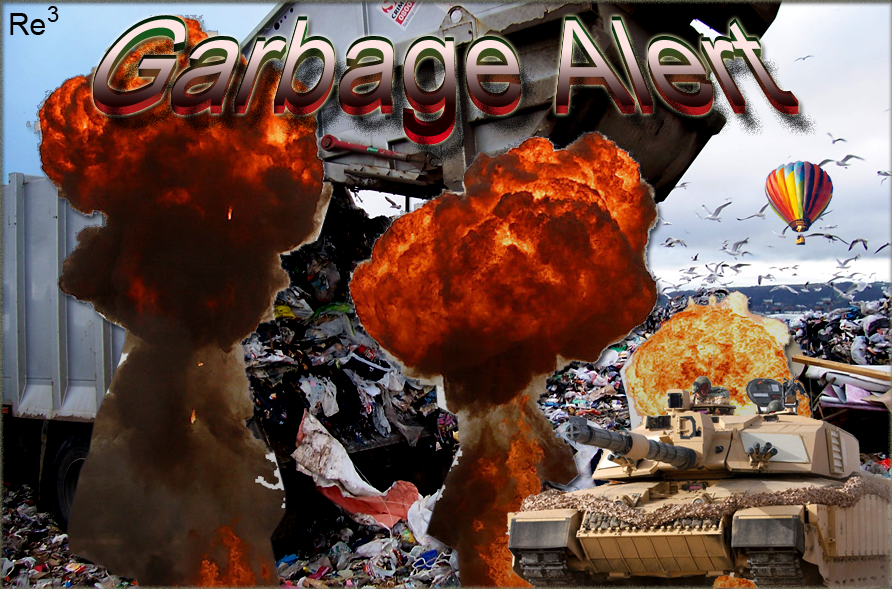
\includegraphics[width=\textwidth]{images/splashscreen.png}
		\caption{Spillets introskjerm}
		\label{fig:splashscreen}
	\end{figure}
\end{center}

\begin{center}
	\begin{figure}
		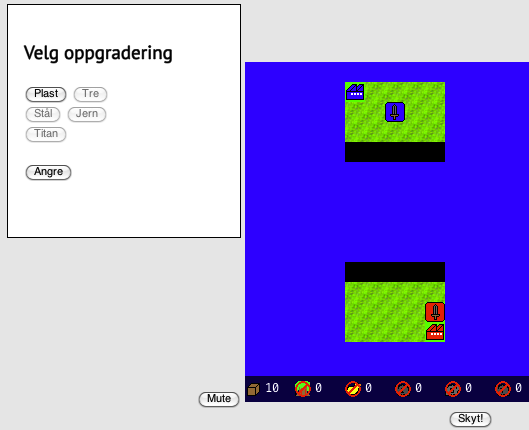
\includegraphics[width=\textwidth]{images/Oppgradering.png}
		\caption{Miljøstasjonen kan oppgraderes til å håndtere ulike typer avfallsgjenvinning.}
		\label{fig:Oppgradering}
	\end{figure}
\end{center}

\begin{center}
	\begin{figure}
		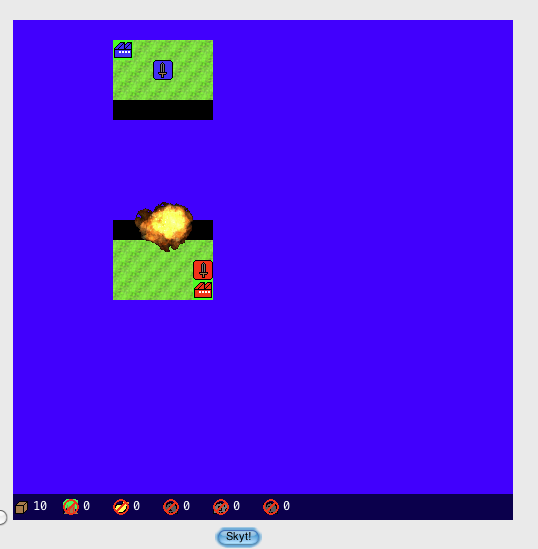
\includegraphics{images/Eksplosjon.png}
		\caption{Ved et angrep på en annen spiller vil et projektil avfyres og eksplodere på motspillerens eventuelle forsvarsstruktur.}
		\label{fig:Eksplosjon}
	\end{figure}
\end{center}

\begin{center}
	\begin{figure}
		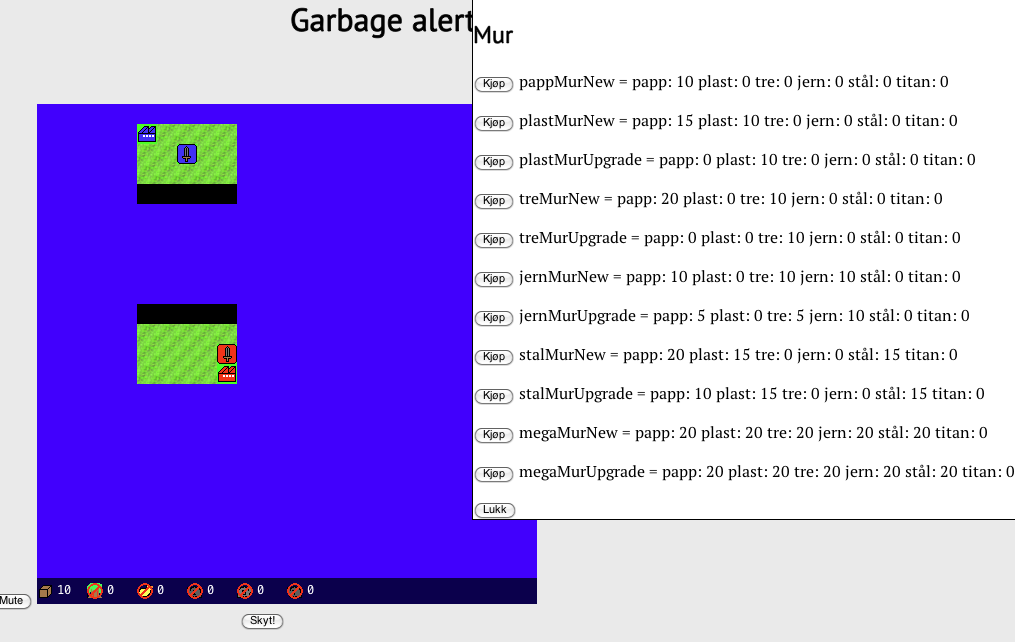
\includegraphics[width=\textwidth]{images/OppgradereMur.png}
		\caption{Spillerens forsvarsstruktur kan oppgraderes til å håndtere sterkere skyts fra motspilleren, avhengig av tilgjengelige ressurser.}
		\label{fig:OppgradereMur}
	\end{figure}
\end{center}

\begin{center}
	\begin{figure}
		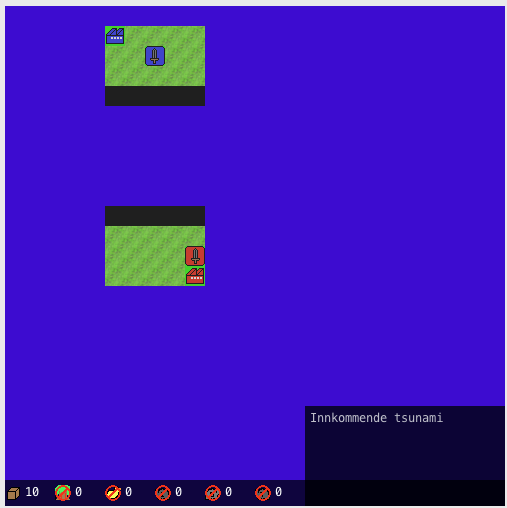
\includegraphics[width=\textwidth]{images/Tsunami.png}
		\caption{Globale geohasarder kan oppstå som følge av mye global forsøpling, som for eksempel en tsunami.}
		\label{fig:Tsunami}
	\end{figure}
\end{center}

\begin{center}
	\begin{figure}
		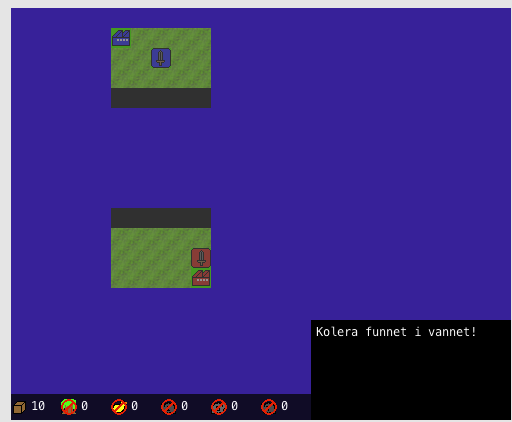
\includegraphics[width=\textwidth]{images/Kolera.png}
		\caption{Lokale biohasarder kan oppstå som følge av mye lokal forurensning. Her er et sykdomsutbrudd.}
		\label{fig:Kolera}
	\end{figure}
\end{center}

\begin{center}
	\begin{figure}
		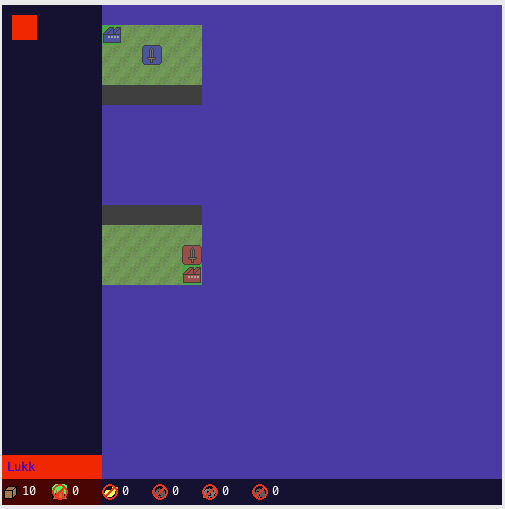
\includegraphics{images/OppgradereEnv.png}
		\caption{Miljøstasjonens effektivitet kan oppgraderes slik at den gjenvinner mer materialer fra hver avfallsenhet.}
		\label{fig:OppgradereEnv}
	\end{figure}
\end{center}



Legg merke til at disse skjermskuddene er tatt av en veldig tidlig prototype som har hatt forkus på å implementere så mye \emph{funksjonalitet} som mulig, heller enn å etablere et konsistent grafisk uttrykk. Vi forsøkte å benytte så mye som mulig av en tidlig prototype videre i den mer avanserte prototypen\footnote{Noen vil kanskje si at dette ble gjort i tråd med landsbyens filosofi om gjenbruk og gjenvinning.}.